%!TEX root = restart.tex
\section{Applications to Optimal coordinated ramp metering on freeways\label{sec:Applications-to-Optimal}}


\subsection{Formulation of the network model and explicit Riemann solver\label{sub:Formulation-of-the}}


\paragraph{Model.}

Consider a freeway section with links $\links=\intrange 1{2\nlinks}$
with a linear sequence of mainline links $=\intrange{2,4}{2\nlinks}$
and connecting onramp links $=\intrange{1,3}{2\nlinks-1}$. At discrete
time $t=\tind\Delta t,0\le\tind\le\ntime-1$, mainline link $2\link\in\links,i\in\intrange 1{\nlinks}$
has a downstream junction $\jdown{2\link}=\jup{2\left(\link+1\right)}$
and an upstream junction $\jup{2\link}=\jdown{2\left(\link-1\right)}$,
while onramp $2\link-1\in\links,i\in\intrange 1{\nlinks}$ has a downstream
junction $\jdown{2\link-1}=\jup{2\link}=\jdown{2\left(\link-1\right)}$
and an upstream junction $\jup{2\link-1}$.

The offramp directly downstream of link $2\link,i\in\intrange 1{\nlinks}$
has, at time-step $\tind$, a split ratio $\splitratio_{2\link}^{\tind}$
representing the ratio of cars which stay on the freeway over the
total cars leaving the upstream mainline of junction $\jdown{2\link}$.
The model assumes that all flux from onramp $2\link-1$ enters downstream
mainline $2\link$. Since $\jup 2$ is the source of the network,
it has no upstream mainline or offramp, and similarly $\jdown{2\nlinks}$
has no downstream mainline or onramp ($\splitratio_{2\nlinks}^{\tind}=0$).
Each link $\link\in\links$ has a discretized state value $\densitydiscrete{\link}{\tind}\in\mathbb{R}$
at each time-step $\tind\in\intrange 0{\ntime-1}$, that represents
the density of vehicles on the link. These values are depicted in
Figure~\ref{fig:Freeway-network-junction}. Junctions that have no
onramps can be effectively represented by adding an onramp with no
demand while junctions with no offramps can be represented by setting
the split ratio to 1.
\begin{figure}
	\begin{centering}
		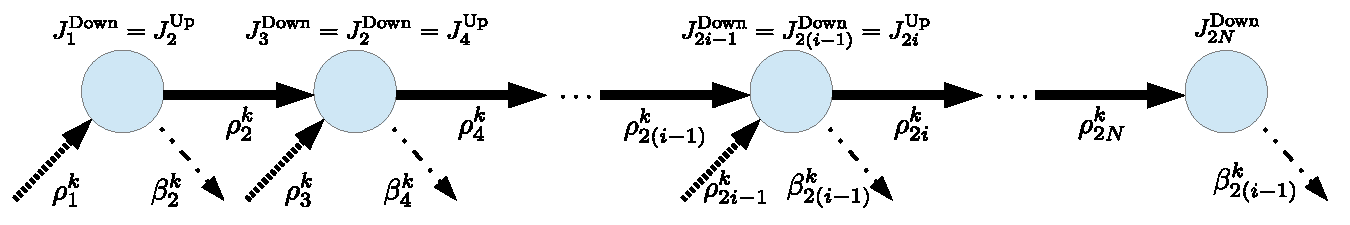
\includegraphics[width=1\columnwidth]{figs-gen/rm-junction-2}
		\par\end{centering}
		
		\caption{Freeway network model. For a junction $\jdown{2\link-1}=\jdown{2\left(\link-1\right)}=\jup{2\link}$
			at time-step $\tind\in\intrange 0{\ntime-1}$, the upstream mainline
			density are represented by $\densitydiscrete{2\left(\link-1\right)}{\tind}$,
			the downstream mainline density by $\densitydiscrete{2\link}{\tind}$,
			the onramp density by $\densitydiscrete{2\link-1}{\tind}$, and the
			offramp split ratio by $\splitratio_{2\left(\link-1\right)}^{\tind}$.\label{fig:Freeway-network-junction}}
		\end{figure}
		
		
		The vehicle flow dynamics on all links $\link$ (mainlines, onramps,
		and offramps) are modeled using the conservation law governing the
		density evolution~\eqref{eq:cons}, where $\density$ is the
		density state, and $f$ is the flux function (or fundamental diagram)
		$f\left(\density\right)$. In the context of traffic, this model is
		referred to as the Lighthill-Whitham-Richards (LWR) model~\cite{lighthill1955kinematic,richards1956shock}.
		The fundamental diagram $f$ is typically assumed to be concave, and
		has a bounded domain $\left[0,\density^{\max}\right]$ and a maximum
		flux value $F^{\max}$ attained at a critical density $\density^{c}:f\left(\density^{c}\right)=F^{\max}$.
		We assume that the fundamental diagram has a trapezoidal form as depicted
		in Figure~\ref{fig:Fundamental-diagram-with}. For the remainder
		of the article, we instantiate the conservation law in~\eqref{eq:cons}
		with the LWR equation as it applies to traffic flow modeling.\begin{wrapfigure}{o}{0.5\columnwidth}%
		\begin{centering}
			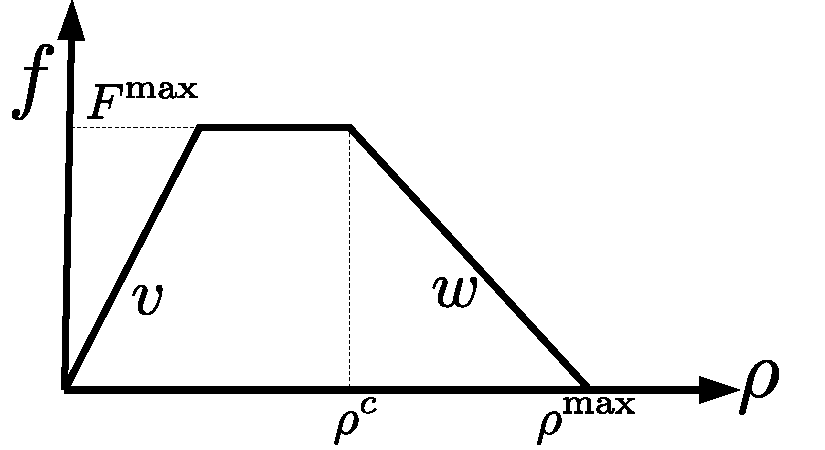
\includegraphics[width=0.4\columnwidth]{figs-gen/fd}
			\par\end{centering}
			
			\caption{Fundamental diagram (the name of the flux function in transportation
				literature) with free-flow speed $v$, congestion wave speed $w$,
				max flux $F^{\max}$, critical density $\density^{c}$, and max density
				$\density^{\max}$.\label{fig:Fundamental-diagram-with}}
			\end{wrapfigure}%
			
			
			As control input, an onramp $2\link-1\in\links,\link\in\intrange 1{\nlinks}$
			at time-step $k\in\intrange 0{\ntime-1}$ has a metering rate $\ramp_{2\link-1}^{\tind}\in\left[0,1\right]$
			which limits the flux of vehicles leaving the onramp. Intuitively,
			the metering rate acts as a fractional decrease in the flow leaving
			the onramp and entering the mainline freeway. The domain of the metering
			control is to force the control to neither impose negative flows nor
			send more vehicles than present in a queue. Its mathematical model
			is expressed in~\eqref{eq:ramp-eqn}.
			
			For notational simplicity we define the set of densities of links
			incident to $\jup{2\link}=\jdown{2\left(\link-1\right)}$ at time-step
			$\tind$ as $\juncstate{\jup{2\link}}{\tind}=\left\{ \discrete{2\left(\link-1\right)}{\tind},\discrete{2i-1}{\tind},\discrete{2\link}{\tind}\right\} $.
			The offramp is considered to have infinite capacity, and thus has
			no bearing on the solution of junction problems. Initial conditions
			are handled as in~\eqref{eq:init-ge}, while for $k\in\intrange 1{\ntime-1}$,
			the mainline density $\discrete{2\link}{\tind}$ using the Godunov
			scheme from~\eqref{eq:main-ge} is given by:
			
			\begin{eqnarray}
				\syseq_{2\link}^{\tind}(\state,\control)= & \discrete{2\link}{\tind}-\discrete{2\link}{\tind-1} & +\dfrac{\Delta t}{\length_{2\link}}\left(\god_{\jdown{2\link}}\left(\juncstate{\jdown{2\link}}{\tind-1},\ramp_{2\link+1}^{\tind-1}\right)\right)_{2\link}\label{eq:rho-update}\\
				&  & -\dfrac{\Delta t}{\length_{2\link}}\left(\god_{\jup{2\link}}\left(\juncstate{\jup{2\link}}{\tind-1},\ramp_{2\link-1}^{\tind-1}\right)\right)_{2\link}\nonumber \\
				= & \discrete{2\link}{\tind}-\discrete{2\link}{\tind-1} & +\frac{\Delta t}{\length_{2\link}}\left(\fout{2\link}{\tind-1}-\fin{2\link}{\tind-1}\right)=0
			\end{eqnarray}
			where we have introduced some substitutions to reduce the notational
			burden of this section: $\fout{\link}{\tind}$ is the Godunov flux
			at time-step $\tind$ exiting a link $\link$ at the downstream boundary
			of the link, and $\fin{\link}{\tind}$ is the Godunov flux entering
			the link at the upstream boundary.
			
			We also make the assumption that onramps have infinite capacity and
			a free-flow velocity $\ffspeed_{2\link-1}=\frac{\length_{2\link-1}}{\Delta t}$
			to prevent the ramp congestion from blocking demand from ever entering
			the network. Since the onramp is has no physical length, the length
			is chosen arbitrarily and the ``virtual'' velocity chosen above
			is chosen to replicate the dynamics in~\cite{Monache2013}. We can
			then simplify the onramp update equation to be:
			
			\begin{eqnarray}
				\syseq_{2\link-1}^{\tind}(\state,\control) & = & \discrete{2\link-1}{\tind}-\discrete{2\link-1}{\tind-1}+\frac{\Delta t}{\length_{2\link-1}}\left(\left(\god_{\jup{2\link}}\left(\juncstate{\jup{2\link}}{\tind-1},\ramp_{2\link-1}^{\tind-1}\right)\right)_{2\link-1}-\boundaryDemand{2\link-1}{\tind-1}\right)\label{eq:onramp-update}\\
				& = & \discrete{2\link-1}{\tind}-\discrete{2\link-1}{\tind-1}+\frac{\Delta t}{\length_{2\link-1}}\left(\fout{2\link-1}{\tind-1}-\boundaryDemand{2\link-1}{\tind-1}\right)=0
			\end{eqnarray}
			where $\boundaryDemand{2\link-1}{\tind-1}$ is the onramp \emph{flux
			}demand, and the same notational simplification has been used for
			the downstream flux. This formulation results in ``strong'' boundary
			conditions at the onramps which guarantees all demand enters the network.
			Details on weak versus strong boundary conditions can be found in
			\cite{Monache2013,Walid,strub2006weak,work2010traffic}.
			
			The onramp model in~\eqref{eq:onramp-update} differs from~\cite{Monache2013,Walid}
			in that we model the onramp as a discretized PDE with an infinite
			critical density, while~\cite{Monache2013,Walid} models the onramp
			as an ODE ``buffer''. While both models implement strong boundary
			conditions, the discretized PDE model makes the freeway network more
			aligned with the PDE network framework presented in this article.
			
			
			\paragraph{Riemann solver.}
			
			For the ramp metering problem, there are many potential Riemann solvers
			that satisfy the properties required in Section~\ref{sub:Network-of-PDE's}.
			Following the model of \cite{Walid,ML}, for each junction $\jup{2\link}$,
			we add two modeling decisions:
			\begin{enumerate}
				\item The flux solution maximizes the outgoing mainline flux $\fin{2\link}{\tind}$.
				\item Subject to (1), the flux solution attempts to satisfy $\fout{2\left(\link-1\right)}{\tind}=p_{2(\link-1)}\fout{2\link-1}{\tind}$,
				where $p_{2(\link-1)}\in\mathbb{R}_{+}$ is a merging parameter for
				junction $\jdown{2\left(\link-1\right)}$. Since (1) allows multiple
				flux solutions at the junction, (2) is necessary to obtain a unique
				solution.
			\end{enumerate}
			This leads to the following system of equations that gives the flux
			solution of the Riemann solver at time-step $k\in\intrange 1{\ntime-1}$
			and junction $\jup{2\link}$ for $\link\in\intrange 1{\nlinks}$:
			
			\begin{eqnarray}
				\demand_{2\left(\link-1\right)}^{\tind} & = & \min\left(\ffspeed_{2\left(i-1\right)}\densitydiscrete{2\left(\link-1\right)}{\tind},F_{2\left(\link-1\right)}^{\max}\right)\label{eq:first-ramp}\\
				\supply_{2\link}^{\tind} & = & \min\left(\congspeed_{2i}\left(\density_{2i}^{\max}-\densitydiscrete{2\link}{\tind}\right),F_{2i}^{\max}\right)\label{eq:supply}\\
				\rampDemand_{2\link-1}^{\tind} & = & \ramp_{2\link-1}^{\tind}\min\left(\frac{\length_{2\link-1}}{\Delta t}\densitydiscrete{2\link-1}{\tind},F_{2i-1}^{\max}\right)\label{eq:ramp-eqn}\\
				\fin{2\link}{\tind} & = & \min\left(\splitratio_{2\left(\link-1\right)}^{\tind}\demand_{2\left(\link-1\right)}^{\tind}+\rampDemand_{2\link-1}^{\tind},\supply_{2\link}^{\tind}\right)\label{eq:fin}\\
				\fout{2\left(\link-1\right)}{\tind} & = & \begin{cases}
				\demand_{2\left(\link-1\right)}^{\tind} & \frac{p_{2(\link-1)}\fin{2\link}{\tind}}{\splitratio_{2\left(\link-1\right)}^{\tind}\left(1+p_{2(\link-1)}\right)}\ge\demand_{2\left(\link-1\right)}^{\tind}\hfill\text{[Case 1]}\\
				\frac{\fin{2\link}{\tind}-\rampDemand_{2\link-1}^{\tind}}{\splitratio_{2\left(\link-1\right)}^{\tind}} & \frac{\fin{2\link}{\tind}}{1+p_{2(\link-1)}}\ge\rampDemand_{2\link-1}^{\tind}\hfill\text{[Case 2}]\\
				\frac{p_{2(\link-1)}\fin{2\link}{\tind}}{\left(1+p_{2(\link-1)}\right)\splitratio_{2\left(\link-1\right)}^{\tind}} & \text{otherwise}\hfill[\text{Case 3]}
				\end{cases}\label{eq:merge}\\
				\fout{2\link-1}{\tind} & = & \fin{2\link}{\tind}-\splitratio_{2\left(\link-1\right)}^{\tind}\fout{2\left(\link-1\right)}{\tind}\label{eq:last-ramp}
			\end{eqnarray}
			where, for notational simplicity, at the edges of of the range for
			$\link$, any undefined state values (e.g. $\densitydiscrete 0{\tind}$)
			are assumed to be zero by convention. Equations~(\eqref{eq:first-ramp})
			and~\eqref{eq:ramp-eqn} determine the maximum flux that can exit
			link $2(\link-1)$ and link $2\link-1$ respectively. Equation~(\eqref{eq:supply})
			gives the maximum flux allowed into link $2\link$. The actual flux
			into link $2\link$, shown in~\eqref{eq:fin}, is given as the minimum
			of the ``demand'' from upstream links and ``supply'' of the downstream
			link. See~\cite{Monache2013} for more details on the model for this
			equation. The flux out of link $2(\link-1)$ is split into three cases
			in~\eqref{eq:merge}. The solutions are depicted in Figure~\ref{fig:Godunov-junction-flux},
			which demonstrates how the flux solution depends upon the respective
			demands and the merging parameter $p_{2\left(\link-1\right)}$. Finally,
			Equation~(\eqref{eq:last-ramp}) gives the flux out of the onramp $2\link-1$,
			which is the difference between the flux into link $2\link$ and the
			flux out of link $2\left(\link-1\right)$ the remains on the mainline.
			\begin{figure}
				\subfloat[Case 1: Priority violated due to limited upstream mainline demand
					entering downstream mainline.]{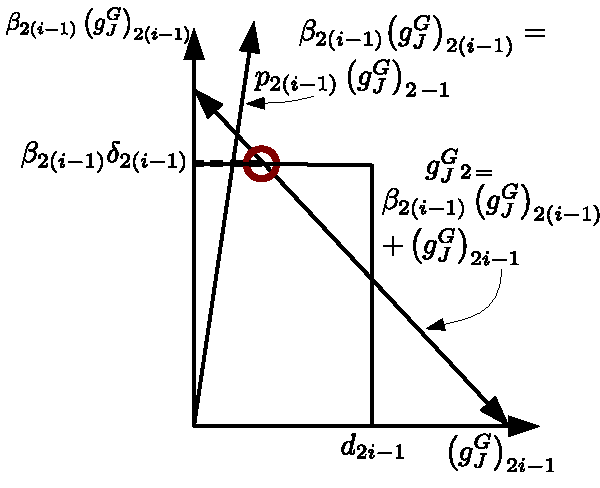
\includegraphics[width=0.3\columnwidth]{figs-gen/flux-sln-1}
							
							}\hfill{}\subfloat[Case 2: Priority violated due to limited onramp demand entering downstream
						mainline.]{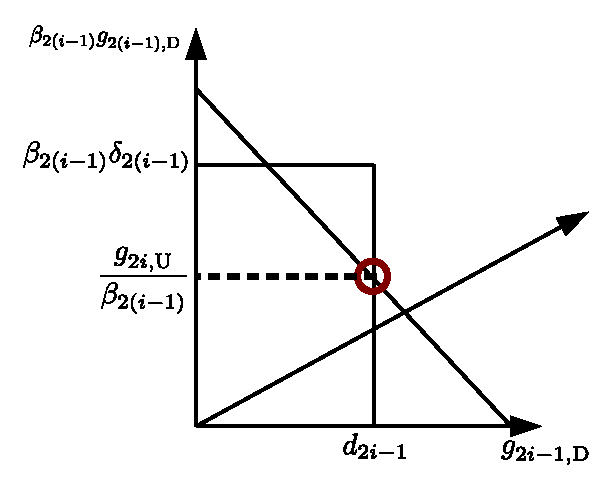
\includegraphics[width=0.3\columnwidth]{figs-gen/flux-sln-2-slim}
								
								}\hfill{}\subfloat[Case 3: Priority rule satisfied due to sufficient demand from both
							mainline and onramp.]{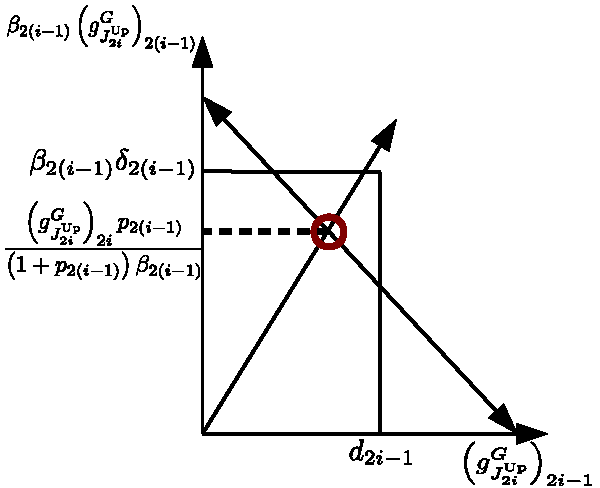
\includegraphics[width=0.3\columnwidth]{figs-gen/flux-sln-3-slim}
									
								}
								
								\caption{Godunov junction flux solution for ramp metering model at junction
									$\jup{2\link}$. The rectangular region represents the feasible flux
									values for $\splitratio_{2\left(\link-1\right)}\fout{2\left(\link-1\right)}{}$
									and $\fout{2\link-1}{}$ as determined by the upstream demand, while
									the line with slope\label{fig:Godunov-junction-flux} $\frac{1}{\splitratio_{2\left(\link-1\right)}}$
									represents feasible flux values as determined by mass balance. The
									$\splitratio_{2\left(\link-1\right)}\fout{2\left(\link-1\right)}{}$
									term accounts for only the flux out of link $2\left(\link-1\right)$
									that stays on the mainline. The flux solution, represented by the
									red circle, is the point on the feasible region that minimizes the
									distance from the priority line $\splitratio_{2\left(\link-1\right)}\fout{2\left(\link-1\right)}{}=p_{2(\link-1)}\fout{2\link-1}{}$.}
							\end{figure}
							
							
							For $\tind=0$, the update equation is given by a pre-specified initial
							condition, as in~\eqref{eq:init-ge}. Note that the equations can
							be solved sequentially via forward substitution. Also, we do not include
							the flux result for offramps explicitly here since its value has no
							bearing on further calculations, and we will henceforth ignore its
							calculation. To demonstrate that indeed the flux solution satisfies
							the flux conservation property, the offramp flux is trivially determined
							to be $\splitratio_{2\left(\link-1\right)}^{\tind}\fout{2\left(\link-1\right)}{\tind}$.
							
							
							\subsection{Formulation of the optimal control problem}
							
							
							\paragraph{Optimal coordinated ramp-metering.}
							
							Including the initial conditions as specified in~\eqref{eq:init-ge}
							with~\eqref{eq:rho-update} and~\eqref{eq:onramp-update} gives
							a complete description of the system $\sys\left(\state,\control\right)=0$,
							$\state\in\mathbb{R}^{2\nlinks}$, $\control\in\mathbb{R}$, where:
							
							\begin{eqnarray*}
								\state_{2\nlinks\tind+\link}\defeq & \densitydiscrete{\link}{\tind} & 1\le i\le2\nlinks,0\le k\le T-1\\
								\control_{\nlinks\tind+\link}\defeq & \ramp_{2\link}^{\tind} & 1\le i\le\nlinks,0\le k\le T-1
							\end{eqnarray*}
							
							
							The objective of the control is to minimize the \emph{total travel
								time }on the network, expressed by the cost function $\cost$:
							
							\[
								\cost\left(\state,\control\right)=\Delta t\sum_{k=1}^{T}\sum_{i=1}^{2\nlinks}L_{i}\densitydiscrete{\link}{\tind}
							\]
							
							
							The optimal coordinated ramp-metering problem can be formulated as
							an optimization problem with PDE-network constraints:
							
							\begin{eqnarray}
								\min_{\control} & \cost\left(\state,\control\right)\label{eq:full}\\
								\text{subject to:} & \sys\left(\state,\control\right) & =0\nonumber \\
								& 0\le\convar\le1 & \forall\convar\in\control\nonumber 
							\end{eqnarray}
							Since the adjoint method in Section~\ref{sec:Adjoint-method} only
							deals with equality constraints, we add barrier penalties to the cost
							function~\cite{Boyd2010,Bayen2006}:
							
							\begin{equation}
								\tilde{\cost}\left(\state,\control,\epsilon\right)=\cost\left(\state,\control\right)-\barrierTerm\sum_{\convar\in\control}\log\left(\left(1-\convar\right)\left(\convar-0\right)\right)\label{eq:full-tilde}
							\end{equation}
							
							
							As $\barrierTerm\in\mathbb{R}^{+}$ tends to zero, the solution to~\eqref{eq:full-tilde}
							will approach the solution to the original problem~\eqref{eq:full}.
							Thus we can solve~\eqref{eq:full} by iteratively solving the augmented
							problem:
							
							\begin{eqnarray}
								\min_{\control} & \tilde{\cost}\left(\state,\control,\epsilon\right)\label{eq:full-1}\\
								\text{subject to:} & \sys\left(\state,\control\right) & =0\nonumber 
							\end{eqnarray}
							
							
							with decreasing values of $\barrierTerm$. As a result, $\tilde{\cost}$
							will approach $\cost$ as the number of iterations increases.
							
							
							\paragraph{Applying the adjoint method.}
							
							To use the adjoint method as described in Section~\ref{sec:Adjoint-method},
							we need to compute the partial derivative matrices $\Hx$, $\Hu$,
							$\tilde{C}_{\state}$ and $\tilde{C}_{\control}$. Computing the partial
							derivatives with respect to the cost function is straight forward:
							
							\begin{eqnarray*}
								\pfrac{\tilde{\cost}}{\discrete{\link}{\tind}}= & \Delta tL_{i} & 1\le i\le2\nlinks,0\le k\le T-1\\
								\pfrac{\tilde{\cost}}{\ramp_{2\link}^{\tind}}= & \barrierTerm\left(\frac{-1}{1-\ramp_{2\link}^{\tind}}+\frac{1}{\ramp_{2\link}^{\tind}}\right) & 1\le i\le\nlinks,0\le k\le T-1
							\end{eqnarray*}
							
							
							To compute the partial derivatives of $\sys$, we follow the procedure
							in Section~\ref{par:Calculating-the-gradient}. For an upstream junction
							$\jup{2\link}\in\jns$ and time-step $k\in\intrange 1{\ntime-1}$,
							we only need to compute the partial derivatives of the flux solver
							$\god_{\jup{2\link}}\left(\juncstate{\jup{2\link}}{\tind},\ramp_{2\link-1}^{\tind}\right)_{\text{}}$
							with respect to the adjacent state variables $\juncstate{\jn_{\link}}{\tind}$
							and ramp metering control $\ramp_{\link}^{\tind}$. We calculate the
							partial derivatives of the functions in~(\eqref{eq:first-ramp})-(\eqref{eq:last-ramp})
							with respect to either a state or control variable$s\in\state\cup\control$:
							
							\begin{eqnarray*}
								\pfrac{\demand_{2\left(\link-1\right)}^{\tind}}s & = & \begin{cases}
								\ffspeed_{2\left(i-1\right)} & s=\densitydiscrete{2\left(\link-1\right)}{\tind},\ffspeed_{i}\densitydiscrete{2\left(\link-1\right)}{\tind}\le F_{2\left(i-1\right)}^{\max}\\
								0 & \text{otherwise}
								\end{cases}\\
								\pfrac{\supply_{2\link}^{\tind}}s & = & \begin{cases}
								-\congspeed_{2i} & s=\densitydiscrete{2\link}{\tind},\congspeed_{2i}\left(\density_{2i}^{\max}-\densitydiscrete{2\link}{\tind}\right)\le F_{2i}^{\max}\\
								0 & \text{otherwise}
								\end{cases}\\
								\pfrac ds & = & \begin{cases}
								\ramp_{2\link-1}^{\tind} & s=\densitydiscrete{2\link-1}{\tind},\densitydiscrete{2\link-1}{\tind}\le F_{2\link-1}^{\max}\\
								\min\left(\densitydiscrete{2\link-1}{\tind},F_{2i-1}^{\max}\right) & s=\ramp_{2\link-1}^{\tind}\\
								0 & \text{otherwise}
								\end{cases}\\
								\pfrac{}s\fin{2\link}{\tind} & = & \begin{cases}
								\splitratio_{2\left(\link-1\right)}^{\tind}\pfrac{\demand_{2\left(\link-1\right)}^{\tind}}s+\pfrac{\rampDemand_{2\left(\link-1\right)}^{\tind}}s & \splitratio_{2\left(\link-1\right)}^{\tind}\demand_{2\left(\link-1\right)}^{\tind}+\rampDemand_{2\link-1}^{\tind}\le\supply_{2\link}^{\tind}\\
								\pfrac{\supply_{2\link}^{\tind}}s & \text{otherwise}
								\end{cases}\\
								\pfrac{}s\fout{2\left(\link-1\right)}{} & = & \begin{cases}
								\pfrac{\demand_{2\left(\link-1\right)}^{\tind}}s & \frac{\fin{2\link}{\tind}p_{2(\link-1)}}{1+p_{2(\link-1)}}\ge\frac{\demand_{2\left(\link-1\right)}^{\tind}}{\splitratio_{2\left(\link-1\right)}^{\tind}}\\
								\frac{1}{\splitratio_{2\left(\link-1\right)}^{\tind}}\left(\pfrac{}s\fin{2\link}{\tind}-\pfrac{\rampDemand_{2\link-1}^{\tind}}s\right) & \frac{\fin{2\link}{\tind}}{1+p_{2(\link-1)}}\ge\rampDemand_{2\left(\link-1\right)}^{\tind}\\
								\frac{p_{2(\link-1)}}{\splitratio_{2\left(\link-1\right)}^{\tind}\left(1+p_{2(\link-1)}\right)}\pfrac{}s\fin{2\link}{\tind} & \text{otherwise}
								\end{cases}\\
								\pfrac{}s\fout{2\link-1}{} & = & \pfrac{}s\fin{2\link}{\tind}-\splitratio_{2\left(\link-1\right)}^{\tind}\pfrac{}s\fout{2\left(\link-1\right)}{}
							\end{eqnarray*}
							
							
							These expressions fully quantify the partial derivative values needed
							in~\eqref{eq:dhdugod} and~\eqref{eqdhdvgod}. Thus we can construct
							the $\Hx$ and $\Hu$ matrices. With these matrices and $\Jx$ and
							$\Ju$, we can solve for the adjoint variable $\lambda\in\mathbb{R}^{2\nlinks\ntime}$
							in~\eqref{eq:adjoint} and substitute its value into~\eqref{eq:adjoint-grad}
							to obtain the gradient of the cost function $\cost$ with respect
							to the control parameter $\control$.
